\pdfoutput=1
% troncons, the short article (English version): the entry door to the three volumes.
% Engine: pdflatex + BibTeX, as arXiv requires (arXiv supports pdflatex; it does not list LuaLaTeX).
% Build: memoire/article/construire-article.sh (figures by lualatex from the judged macros of Volume III,
% then pdflatex, bibtex, and pdflatex three times). arXiv package: this folder's .tex, .bbl and
% troncons-figures.pdf (see memoire/article/REPRISE-article.md).
% Every number comes from a committed file, named in the text, in a table's source line or in a comment.
\documentclass[11pt, a4paper]{article}
\usepackage[T1]{fontenc}
\usepackage[utf8]{inputenc}
\usepackage[english]{babel}
\usepackage{amsmath, amsthm}
\usepackage{libertinus}
\usepackage{libertinust1math} % Libertinus for the mathematics too, as in the figures (no amssymb: this package gives \mathbb)
\usepackage[a4paper, left=22mm, right=22mm, top=22mm, bottom=26mm]{geometry} % text width 166 mm; the figures were judged at 156 mm
\usepackage{microtype}
\usepackage{graphicx, booktabs, tabularx, array}
\usepackage{xcolor}
\usepackage[group-separator={\,}, group-minimum-digits=4]{siunitx}
\usepackage[numbers, sort&compress]{natbib}
\usepackage[font=small, labelfont={sf,bf}]{caption}
\usepackage{enumitem}
\setlist{nosep, leftmargin=*, topsep=3pt}
\usepackage[normalem]{ulem}
\usepackage{xurl}
\definecolor{Accent}{HTML}{1F5C99}
\usepackage[colorlinks=true, linkcolor=Accent, citecolor=Accent, urlcolor=Accent, pdfusetitle]{hyperref}
\usepackage[capitalise, noabbrev]{cleveref}

% Floats: fewer pages of figures alone; a compact bibliography.
\renewcommand{\topfraction}{0.9}
\renewcommand{\bottomfraction}{0.6}
\renewcommand{\textfraction}{0.07}
\renewcommand{\floatpagefraction}{0.8}
\setlength{\bibsep}{1.5pt}
\renewcommand{\bibfont}{\footnotesize}

\newtheorem{proposition}{Proposition}
\newtheorem{corollary}[proposition]{Corollary}
\newtheorem{lemma}[proposition]{Lemma}
\theoremstyle{remark}
\newtheorem{remark}[proposition]{Remark}

% Provenance of a number, as in the three volumes.
\newcommand{\etiq}[1]{\textsf{\scriptsize[#1]}}
\newcommand{\mes}{\etiq{meas.}}
\newcommand{\calc}{\etiq{calc.}}
\newcommand{\litt}{\etiq{lit.}}
\newcommand{\fichier}[1]{\textsf{\footnotesize\nolinkurl{#1}}}
\newcommand{\source}[1]{\par\smallskip{\footnotesize\textit{Source:} #1\par}}
\newcommand{\barre}[1]{\sout{#1}}
\newcommand{\Prob}{\mathbb{P}}
% Used by the bibliography (memoire/article/commun/troncons-article.bib).
\newcommand{\Consulte}[1]{Accessed #1}
\newcommand{\RapportTechnique}{Technical report}
\newcommand{\Emplacement}{\textit{[location to be filled in]}}
\newcommand{\NoteTome}{English and French versions; \Emplacement}
% The titles of the three volumes, as on their title pages (memoire/commun/page-titre.tex,
% memoire/tome2/en/troncons-tome2-en.tex, memoire/tome3/en/troncons-tome3-en.tex), in the language of the paper.
\newcommand{\TitreTomeI}{troncons: running a model far larger than memory. Research thesis, Parts I and II: the measured foundations (Volume~I)}
\newcommand{\TitreTomeII}{troncons, Volume II: the system}
\newcommand{\TitreTomeIII}{troncons, Volume III: the genome of the weights}
% The figures: pages of troncons-figures.pdf, drawn from the judged macros of Volume III.
% #1 page; #2 width as a fraction of 156 mm, the width at which Volume III's judges saw them (only the size changes).
\newcommand{\Figure}[2]{\includegraphics[page=#1, width=#2\dimexpr 156mm\relax]{troncons-figures}}

\title{Sixteen codes for fifteen values: a lossless synonymous codon in MXFP4,\texorpdfstring{\\}{ }
and gpt-oss-120b served from disk on a \texorpdfstring{16\,GB}{16 GB} laptop}
\author{Stone}
\date{29 October 2026}

\begin{document}
\maketitle

\begin{abstract}
MXFP4, the 4-bit format in which gpt-oss publishes its expert weights, has sixteen codes for fifteen values: $+0$ and $-0$ are two codes of the same zero. The quantiser of gpt-oss keeps the sign of values rounded to zero; over the \num{19110297600} expert weights of gpt-oss-20b, that sign is a fair coin (entropy 0.9999999967 bit), and no computation of the engines considered depends on it. We prove that folding $-0$ into $+0$ before entropy coding saves exactly $\Prob(V = 0)\,H(S \mid V = 0)$ bit per weight, twice the share of $-0$ codes when the sign is a fair coin, and we check it on all 180 expert tensors of gpt-oss-20b and gpt-oss-120b to within $1.7 \times 10^{-4}$ bit. Carried into version 1.2 of the \texttt{.trc} format of the troncons engine by its coding tables alone, decoder and kernels unchanged, the fold removes \num{1800486912} bytes (1.80\,GB) from gpt-oss-120b, 0.12562 bit per expert weight (3.26\,\% of its bits), and the engine's logits stay identical to the bit over \num{5120} steps on both models. troncons serves gpt-oss-120b (63.4\,GB) on a laptop with 16\,GB of RAM and an 8\,GB RTX\,4060, with a host working set of 384\,MB and a GPU footprint set by the card, not by the model (about 6.3\,GB of its 8\,GB). On this laptop, in an ABBA series, the v1.2 file generates 2.890 tokens/s against 1.988 for v1.0 ($\times 1.454$; an independent judge: $\times 1.442$), whereas its 3.3\,\% fewer bytes would allow at most $+3.4\,\%$: a crossed experiment on gpt-oss-20b, at the disk stage, shows that the gain follows the pattern of read requests that the format imposes on this disk. It is a result of this machine, not a portable one. We also report what did not work, each against its declared threshold, and the method: thresholds committed before measuring, controls that can fail, independent judges.
\end{abstract}

% =============================================================================================================
\section{Introduction}\label{sec:intro}

The project behind this paper set itself a concrete goal: run, on an ordinary laptop, a language model much larger than all of the laptop's memory, \emph{exactly} (to the bit, the logits that the same engine computes from the uncompressed weights), by storing its weights compressed on disk and decoding only what a computation needs, at the moment it needs it. The machine has 16\,GB of RAM, an RTX\,4060 Laptop GPU with 8\,GB, and a 1\,TB NVMe disk encrypted by BitLocker. The model is gpt-oss-120b \citep{openai2025gptoss}, a mixture of experts of 63.4\,GB in its native MXFP4 format: four times the RAM, eight times the GPU memory.

Three technical volumes report the work in full, each in English and French. Volume~I \citep{troncons-tome1} measured the machine and showed that, on it, everything comes down to the number of bits read from disk per weight. Volume~II \citep{troncons-tome2} built the engine, troncons, and judged its first milestone (J1) against twelve criteria declared before the first line of code. Volume~III \citep{troncons-tome3} searched for a way to read fewer bits and built what held. This short paper is their entry door. It reports one small, exact idea and what it did on this machine, and it says plainly what did not work.

The idea is a synonym. In the genetic code, several codons give the same amino acid \citep{crick1968}; in MXFP4, two codes give the same zero. When the sign of a zero carries no information, which is the case in gpt-oss, storing it costs almost one bit per zero, and about one expert weight in eight is a zero. Removing it is lossless as long as every reader of the codes reads both codes as zero, and that is a property one can prove on the real kernel. The spare code of zero is known, and other formats give it another value (\cref{sec:travaux}); we do not, because we keep the model as it was published, every weight with the same value, and only stop paying for a sign that changes no value.

\paragraph{Contributions.}
\begin{itemize}
\item A measurement, tensor by tensor on the 180 expert tensors of two published models, that the sign of a zero is a fair coin, and the exact, elementary statement of what folding the synonym saves, $H(C) = H(V) + \Prob(V = 0)\,H(S \mid V = 0)$ (\cref{sec:codon,sec:res-gain}).
\item A proof that the engine's MXFP4 matrix--vector kernel returns the same bits on both codes, and a lemma showing that the fold is carried into a format through its coding tables, with no change to the decoder (\cref{sec:codon,sec:format}).
\item The \texttt{.trc} v1.2 files of gpt-oss-20b and gpt-oss-120b, checked expert by expert in value, 1.80\,GB smaller on the 120b, with logits identical to the bit (\cref{sec:res-taille,sec:res-exact}).
\item Milestone J1 redone on gpt-oss-120b in ABBA series, and an attribution of its $\times 1.45$ to the read pattern of the format on this disk, by a crossed experiment of an independent judge on gpt-oss-20b, at the disk stage (\cref{sec:res-j1,sec:res-motif}).
\item Negative results with their declared thresholds, and the measurement discipline that produced all of the above (\cref{sec:methode-regles,sec:echecs}).
\end{itemize}

Labels follow the volumes: \mes{} measured on this machine, tool and log committed; \calc{} computed from committed measurements; \litt{} literature, not reproduced. Paths such as \fichier{genome/06-codon-v1-2.md} are relative to the troncons repository (\cref{sec:dispo}).

% =============================================================================================================
\section{Related work}\label{sec:travaux}

\paragraph{Serving models larger than memory.} FlexGen offloads weights and cache across GPU, CPU and disk to maximise the throughput of batched generation with a single GPU \citep{flexgen2023}. LLM in a Flash reads weights from flash storage on demand, with windowing and row--column bundling to enlarge reads \citep{llminflash2024}. PowerInfer splits neurons into a hot set kept on the GPU and a cold set computed on the CPU \citep{powerinfer2024}. For mixtures of experts, \citet{mixtraloffload2023} keep an LRU cache of experts on the GPU and load others speculatively; MoE-Infinity designs an expert cache for personal machines \citep{moeinfinity2024}; Fiddler computes cold experts on the CPU instead of moving them \citep{fiddler2025}. llama.cpp offloads MoE layers between host and GPU and is the baseline of Volume~II \citep{llamacpp2026b11515}. troncons differs in its contract: weights stay \emph{losslessly entropy-coded} on disk and are decoded on the GPU at the moment of use, and the logits are, to the bit, those that the engine computes from the raw GGUF weights; the expert cache and its theory (Belady's optimality \citep{belady1966}, the bounds of LRU) are in Volume~II.

\paragraph{Lossless compression of weights.} ZipNN \citep{hershcovitch2024zipnn}, DFloat11 \citep{zhang2025dfloat11} and Huff-LLM \citep{yubeaton2025huffllm} compress weights without loss, mostly by entropy coding the redundant part of floating-point representations such as BF16 exponents. Lossy sub-bit compression of very large MoEs also exists \citep{frantar2023qmoe}. We work one level lower, inside a format that is already four bits: MXFP4 \citep{ocpmx2023,rouhani2023microscaling} stores blocks of 32 E2M1 codes sharing an E8M0 scale. Its redundancy that we exploit is not statistical skew but a \emph{synonym}: two codes, one value, by the signed zero of IEEE~754 \citep{ieee754}. That redundancy is known. BitMoD replaces the redundant zero of FP3 and FP4 variants by a special value \citep{chen2024bitmod}; the code recycling of NxFP remaps the $-0$ code of sign-magnitude formats to half the smallest quantisation level, and applies it to MXFP4 \citep{lo2024nxfp}; RaZeR remaps the redundant zero of NVFP4 to further quantisation values \citep{chen2025razer}. All three are new, lossy formats into which a model is quantised again, and none measures how often $-0$ occurs in a published model. Lossless coding has been extended to FP8 and FP4 \citep{heilper2025lossless}, but for FP4 it compresses only the block scales and stores the 4-bit values uncompressed, reporting that their streams appear statistically uniform; in gpt-oss-20b, the entropy of the codes is 3.8638 bits per weight, not 4 (\cref{sec:codon}), and our coder conditions them on the scale class. We know of no work that measures, in a model already published in MXFP4, whether the sign of a zero carries information, and removes it without loss, with a proof that the kernel returns the same bits. The entropy coder is interleaved rANS \citep{duda2013ans,giesen2014interleaved}; the information-theoretic tools are standard \citep{cover2006}; the quality judge is the Kullback--Leibler divergence \citep{kullback1951} against a double-precision reference.

\paragraph{Ideas that we tested and that failed.} The router of an MoE layer partitions its input space into polyhedral regions, as a tropical polynomial does \citep{zhang2018tropical}; weight matrices of trained networks often show heavy-tailed spectra \citep{martin2018implicit}, which one tests against a power law by the method of \citet{clauset2009power}. \Cref{sec:echecs} reports what these readings gave on gpt-oss.

% =============================================================================================================
\section{Method}\label{sec:methode}

\subsection{The machine, the model and the engine}\label{sec:moteur}

\paragraph{The machine} \mes. Windows~11, an i7-13620H (16 threads), 16\,GB of RAM (15.6 usable), an RTX\,4060 Laptop GPU with \num{8188}\,MiB on a PCIe~4.0~$\times 8$ link, a 1\,TB Samsung NVMe disk behind Intel RST VMD, under BitLocker. Volume~I measured 2.82\,GB/s from the disk (\fichier{fondations/journaux/01-machine/debits-mesures.json}).

\paragraph{The model} \litt\,\mes. gpt-oss-120b has 36 layers of 128 experts, of which the router of each layer chooses four per token; its GGUF file is \num{63387346208} bytes, its \num{4608} experts 61.07\,GB, and every token also reads 1.69\,GB of attention, routers and output head (\fichier{mesures/gpt-oss.md}). Its development twin, gpt-oss-20b (24 layers of 32 experts, \num{12109566624} bytes), is already larger than the GPU.

\paragraph{The engine and its byte path.} troncons is a Rust workspace with CUDA kernels loaded through the driver API alone (Volume~II, chapters 1 to 6). One \texttt{.trc} file per model, aligned on \num{4096} bytes, holds one \emph{chunk} per expert: the expert's three MXFP4 matrices, entropy-coded by interleaved rANS with 32 lanes, each lane knowing from its position which table to use (one table per scale class $\kappa$), plus a directory with the offset, length and fingerprint of every chunk. The resident weights (attention, routers, head) live in VRAM; experts live in a VRAM cache of fixed slots. When a router asks for an expert that is not in a slot (a miss), its chunk travels four stages:
\begin{enumerate}
\item \textbf{disk to host}: one unbuffered read (\texttt{FILE\_FLAG\_NO\_BUFFERING}) per chunk, issued without waiting and harvested from an I/O completion port \citep{microsoft2025iocp}, straight into pinned host memory;
\item \textbf{host to GPU}: a DMA from that same pinned page over PCIe; the GPU has a single copy engine under WDDM, a fact Volume~II measured;
\item \textbf{decoding}: a CUDA rANS decoder turns the chunk into an expert slot, proved to return exactly the scalar decoding;
\item \textbf{compute}: an MXFP4 matrix--vector kernel (GEMV) reads the slot; every reduction follows a fixed tree, so two runs on the same bytes return the same bits.
\end{enumerate}
A production guard compares the fingerprint of every chunk read with the directory and turns any corruption into a named fatal error. Volume~II's results on gpt-oss-120b, with the v1.0 format: a peak host working set of 384\,MB (\num{384.19}\,MB, pinned memory included, against \num{380.50}\,MB for the 20b, which is five times smaller), where llama.cpp holds 10.93\,GB of host memory in its best published configuration, while troncons's private committed memory, 6.93\,GB (llama.cpp: 6.81\,GB), is, as Volume~II reads it (published there, not judged), of the order of its GPU allocations and pinned memory, reserved against the commit limit of Windows without occupying physical RAM; both engines also use the GPU, troncons about 6.3\,GB of its 8\,GB (\num{6317303600} bytes), a share set by the card, not by the model, and nvidia-smi reads the whole card, other processes included, at a peak of \num{6574}\,MiB under troncons and of \num{6026} and \num{6027}\,MiB under llama.cpp in that configuration (independent trial of Volume~II, \fichier{mesures/moteur/epreuve-J1/csv/s1-2026-10-16-passes.csv}, which also holds the committed memory), so that the large gap between the two engines lies in the host working set; logits identical to the bit between the coded and the raw file over \num{5120} steps, by the same engine; 1.965 tokens/s with the guard, $\times 2.22$ the best llama.cpp configuration measured (0.884 tokens/s; two sessions of the same morning, Volume~II); and, on window 0 (255 positions) with an f16 KV cache, a KL divergence to an f64 reference of 0.00308, against 0.0607 for llama.cpp \mes~(Volume~II, chapter~7; \fichier{mesures/moteur/O/}, \fichier{mesures/moteur/epreuve-J1/}). Volume~II traces most of llama.cpp's gap, on the 20b, to its rounding of the YaRN ramp \citep{peng2023yarn} rather than to kernel precision; with an f32 KV cache, troncons's KL is $-0.00048$, at the resolution floor of the logit files themselves (\texttt{.kld}, $\log q$ on 16 bits). Host memory no longer follows the size of the model.

\subsection{The synonymous codon of zero}\label{sec:codon}

E2M1 has one sign bit and three magnitude bits. llama.cpp and troncons double its magnitudes into the integers $K = (0, 1, 2, 3, 4, 6, 8, 12)$ and move the factor 2 into the scale. For a code $c \in \{0, \dots, 15\}$ with bits $c_3c_2c_1c_0$,
\begin{equation}\label{eq:valeur}
v(c) = (-1)^{c_3}\,K[c \mathbin{\&} 7].
\end{equation}
The map $v$ is injective except on $\{0, 8\}$: $v(0) = +0$ and $v(8) = -0$, and $-0 = +0$ in IEEE~754. Sixteen codes, fifteen values (\cref{fig:roue}).

\begin{figure}[tbp]
\centering
\Figure{1}{0.8}
\caption{\textbf{The fold $8 \to 0$ removes one of the two codes of zero.} The fifteen values of E2M1 at equal steps around a circle (0 at the top; values of the OCP standard, which llama.cpp doubles). The width of a ray grows with the measured share of its code in the 72 expert tensors of gpt-oss-20b (\num{19110297600} weights), affinely (0.4\,pt $+$ 44\,pt $\times$ share), so the zero ray thickens by $\times 1.88$, not $\times 2$. Before: \texttt{0000} ($+0$, 6.3920\,\%) and \texttt{1000} ($-0$, 6.3929\,\%) for one value; after, one ray carries both. The sign of a zero is a fair coin. Analogy, not proof: GGU, GGC, GGA and GGG all give glycine. \mes\ Data: \fichier{mesures/genome/predictif-elagage/histo-toutes-gptoss20b.npz}, \fichier{mesures/genome/etat-de-l-art/journaux/zero-compte-20b.json}.}
\label{fig:roue}
\end{figure}

\paragraph{The coin} \mes. The quantiser of gpt-oss keeps the sign of a value rounded to zero. Over the 72 expert tensors of gpt-oss-20b, the code $+0$ has the share 6.3920\,\% and $-0$ the share 6.3929\,\%: the sign of a zero has an entropy of 0.9999999967 bit. The entropy of the codes is 3.8638 bits per weight, that of the values 3.7360; the difference, 0.1278 bit, is what a sign that changes no value costs (\fichier{mesures/genome/etat-de-l-art/journaux/zero-compte-20b.json}).

\begin{proposition}[Entropy of a code with a synonym]\label{prop:gain}
Let $C$ be the code of a weight, $V = v(C)$ its value and $S = C_3$ its sign bit. Then $H(C) = H(V) + \Prob(V = 0)\,H(S \mid V = 0)$.
\end{proposition}
\begin{proof}
$V$ is a function of $C$, so $H(C, V) = H(C)$, and by the chain rule $H(C, V) = H(V) + H(C \mid V)$. Given $V = v \neq 0$, $C$ is determined, since $v$ is injective away from 0. Given $V = 0$, $C \in \{0, 8\}$ is determined by $S$. Hence $H(C \mid V) = \Prob(V = 0)\,H(S \mid V = 0)$.
\end{proof}

\begin{corollary}[The gain of the fold]\label{cor:gain}
Replacing $C$ by $C' = \gamma(C)$, with $\gamma(8) = 0$ and $\gamma$ the identity elsewhere, makes $C'$ a bijection of $V$, so the entropy falls by $\Prob(V = 0)\,H(S \mid V = 0)$ bit per weight. If the sign of a zero is a fair coin, the $-0$ codes are half of the zeros and
\begin{equation}\label{eq:deuxfois}
\text{gain} = \Prob(V = 0) = 2 \times (\text{share of } {-0} \text{ codes}).
\end{equation}
The same holds conditionally on any context $X$ the decoder knows (scale class, neighbouring byte): replace $H(\cdot)$ by $H(\cdot \mid X)$ throughout. If the context predicted the sign, the gain would be smaller than $\Prob(V = 0)$.
\end{corollary}

\begin{remark}[Bytes]\label{rem:octets}
The coder works on bytes, two codes at a time. The fold removes from the alphabet the bytes one of whose nibbles is 8: $16 + 16 - 1 = 31$ bytes, so $256 - 31 = 225$ remain \calc. Applied to the byte and its pair of values, the same proof gives $\Prob(V = 0)$ bit per weight when the signs of zeros are fair coins, independent of everything else.
\end{remark}

The fold is lossless only if \emph{every} reader of the codes gives code 8 the value 0. The project lists them (\fichier{genome/06-codon-v1-2.md} §\,1): ggml reads the codes through an int8 table where entry 8 is 0 \litt; the GPU decoder copies bytes without reading values; the f64 reference reads the GGUF, not the \texttt{.trc}; and the only reader of values in the engine's kernels is the GEMV, where code 8 is $-0.0$f. The question is therefore that of the \emph{bits} of a sum in which one term goes from $-0$ to $+0$.

\begin{proposition}[The GEMV returns the same bits; Volume~III, Proposition A1]\label{prop:a1}
The engine's MXFP4 GEMV (\fichier{moteur/crates/trc-noyaux/noyaux/gemv.cuh}, in its version of commit \texttt{4473050}, the one in the tree at \texttt{000cef9}) starts each accumulator at $s = +0$ and advances by $s \leftarrow \mathrm{fma}(v, x, s)$ in a fixed order, with $v$ the doubled signed magnitude of the code. If the inputs $x$ are finite, replacing code 8 by code 0 changes no bit of $s$ at any step.
\end{proposition}
\begin{proof}[Sketch]
(0) Every finite binary32 is a multiple of $2^{-149}$ and $v$ is an integer, so every exact sum $v x + s$ lies on the grid $2^{-149}\mathbb{Z}$; if it is not zero, its rounding is not zero. (1) The accumulator is never $-0$: it starts at $+0$; an exact zero sum rounds to $+0$ unless both terms are $-0$, which (by induction) $s$ is not; a non-zero sum does not round to zero by (0). (2) For $v = \pm 0$, $v x = \pm 0$ exactly; if $s \neq 0$, $s' = s$; if $s = 0$ then $s = +0$ and $s' = +0$ whatever the sign of $v x$. (3) Other steps have bit-equal operands. By induction, $s$ is bit-equal in both computations; the fixed-tree reduction then adds bit-equal partial sums, and the scale and bias are applied afterwards.
\end{proof}

The proof uses the fact that magnitudes are doubled to integers and that the scale stays outside the accumulation; a kernel that put the scale inside, or started a GEMM from $-0$, would leave it. The project therefore wrote an invariant into its architecture: every code reader reads code 8 as zero, and every new kernel that reads codes carries a control that compares an expert with its canonicalised copy. The same induction holds for the f64 reference under one hypothesis, stated in Volume~III: no non-zero exact sum underflows to zero.

\subsection{The \texttt{.trc} v1.2 format}\label{sec:format}

The coder canonicalises the codes of each expert ($8 \to 0$) before counting symbols and building its rANS tables, so the 31 bytes that carry a nibble 8 receive frequency zero. Nothing else changes (\cref{tab:format}).

\begin{lemma}[The invariant of the tables suffices]\label{lem:tables}
If the table of a context gives $f[s] = 0$ to a symbol $s$, no stream, correct or corrupted, makes the decoder produce $s$.
\end{lemma}
\begin{proof}
The decoder reads slot $i = x \bmod 4096$ of its state $x$ and returns the symbol that carries it; by construction slot $i$ carries the $s$ with $c[s] \le i < c[s] + f[s]$, $c$ the cumulative frequencies. If $f[s] = 0$ the interval is empty and no slot carries $s$, whatever $x$.
\end{proof}

Two engineering consequences follow. The guarantee ``no v1.2 stream produces a $-0$'' is checked once, on the tables, at opening ($36 \times 3 \times 3 \times 31 = \num{10044}$ reads for the 120b \calc), not per symbol. And \emph{a v1.2 stream is a v1.0 stream whose effective alphabet has 225 bytes}: the GPU decoder and the GEMV have not had a single line changed. A synonym enters a format through its tables, not through its decoder. Because a v1.2 file is no longer bit-equal to the GGUF but equal in value, each directory entry keeps two fingerprints, the original one (provenance) and the canonical one (what the decoder must return), and the verifier compares values, not only bytes.

\begin{table}[tbp]
\centering\small
\caption{What changes from \texttt{.trc} v1.0 to v1.2, and nothing else.}
\label{tab:format}
\begin{tabularx}{\linewidth}{@{}>{\raggedright\arraybackslash}p{0.24\linewidth}l>{\raggedright\arraybackslash}p{0.2\linewidth}>{\raggedright\arraybackslash}X@{}}
\toprule
Where & Offset & v1.0 & v1.2 \\
\midrule
header, minor version & 10 (u16) & 0 & \textbf{2} \\
header, flags & 12 (u32) & bits 0 to 2 & $+$ \textbf{bit 3, canonical} \\
directory, each entry & 56 (u64) & reserved, 0 & fingerprint of the canonical expert \\
CODES\_CTX tables & --- & 256 frequencies & built on canonical codes; frequency 0 for the 31 bytes that carry an 8, checked at opening \\
\bottomrule
\end{tabularx}
\source{\fichier{decisions/ARCHITECTURE.md} §\,4.16; \fichier{genome/06-codon-v1-2.md} §\,2. The reader refuses bit 3 under a minor version below 2, on a raw or two-level file, a canonical fingerprint without bit 3, and a canonical table that gives a slot to a byte carrying an 8; each refusal has its test and its break.}
\end{table}

\begin{figure}[tbp]
\centering
\Figure{2}{0.9}
\caption{\textbf{After the fold, row and column 8 go out: 225 bytes remain of 256.} The CODES\_CTX table ($\kappa = 1$) of gpt-oss-120b, layer 18, up matrix, as a $16 \times 16$ grid (high nibble in rows, low nibble in columns); grey level $\log_{10}(1 + f)$, $f$ the frequency out of \num{4096}. Framed white cells: frequency zero, absent. Their mass moves onto row and column 0. Over all 540 CODES\_CTX tables of both models, a second reader written from the specification alone finds a slot for a byte carrying an 8 in 540 v1.0 tables (13\,\% of the slots on average) and in none of the v1.2 tables. \mes\ Data: \fichier{mesures/genome/construction/codon/tables-octets.csv}, \fichier{tables-octets.json}.}
\label{fig:octets}
\end{figure}

\subsection{How the measurements were made}\label{sec:methode-regles}

The numbers of this paper were produced under rules that the project applies to every step, and that matter as much as the numbers.
\begin{itemize}
\item \textbf{Thresholds declared before measuring.} Each criterion and its threshold are written and committed before the first pass; the threshold derives from a named, measured quantity. The criteria of the v1.2 step (A-C1 logits, A-C2 size, A-C3 speed) are in the header of \fichier{outils/genome/construction/codon/pilote\_codon.py}, commit \texttt{a50c380}, before any pass; the amendment of the calm session s2 is commit \texttt{71905dd}, before its passes.
\item \textbf{Controls that can fail, and breaks.} Every measurement has a control whose answer is known in advance, and every new control is broken on purpose to check that the instrument falls. Examples: a coder run without the new option must write v1.0 byte for byte (same SHA-256 as the file of 15 October); a falsified median in one expert must make the logits differ (512 rows out of 512); a nibble 0 changed into 8 in a decoded expert must fail the byte checks and pass the value check.
\item \textbf{ABBA series.} A cost is never based on one pass: fresh processes alternate A B B A A B B A, and the noise is the spread of a program against itself. A gain is announced only if $r - 1 > 2\sigma$, $\sigma$ the relative standard deviation of the A passes; no regression is declared if $r \ge 1 - 2\sigma$. Passes run on mains power, under a lock on the GPU, and are discarded if another process loaded the machine (more than 5\,\% of a core or 8\,MB read in 3\,s).
\item \textbf{Independent judges.} Each step is redone by a judge who wrote neither the decision nor the code, with their own tools: here, a decoder of the format written from its description alone, a GGUF reader, fresh text windows nobody had seen, a three-file speed session, and a disk reader of their own.
\item \textbf{Strike-throughs.} When a measurement contradicts a published sentence, even our own, the sentence is struck through where it stands and what changed is written next to it. This paper carries one such correction (\cref{sec:res-motif}).
\end{itemize}

% =============================================================================================================
\section{Results}\label{sec:resultats}

\subsection{The gain, tensor by tensor}\label{sec:res-gain}

The coder folded \num{1221698587} nibbles 8 on gpt-oss-20b (6.393\,\% of its expert weights) and \num{7199491948} on gpt-oss-120b (6.279\,\%); the verifier, which canonicalises the slices of the GGUF by its own path, counts the same numbers to the unit \mes~(\fichier{genome/06-codon-v1-2.md} §\,5). \Cref{cor:gain} therefore predicts $2 \times 0.0639288 = 0.12786$ bit (20b) and $2 \times 0.0627889 = 0.12558$ bit (120b); the gain measured on the coded chunks is 0.12791 and 0.12562 bit \calc. On each of the 180 expert tensors (72 of the 20b, 108 of the 120b), the gap between the measured gain and twice the share of $-0$ codes lies between $-0.00017$ and $+0.00016$ bit, $+0.00005$ on average (\cref{fig:theoreme}). This is stronger than it looks: had the scale class or the neighbouring byte, both known to the coder, predicted the sign of a zero, the measured gain would fall below $\Prob(V = 0)$. In every tensor, the sign of a zero is a fair coin that neither the scale class nor the other nibble of its byte predicts, and the rANS coder recovers its whole bit. The gain ranges from 0.115 bit (120b, layer 26, up) to 0.239 bit (120b, layer 0, up, where 11.9\,\% of the weights are $-0$).

\begin{figure}[tbp]
\centering
\Figure{3}{0.78}
\caption{\textbf{The 180 expert tensors of the two models sit on the diagonal that \cref{cor:gain} predicts.} (a) Measured gain of the fold (bits per expert weight, code streams of each tensor) against twice the share of $-0$ codes; the two points of layer 0 of the 120b are the richest in zeros. (b) Measured minus predicted, in $10^{-4}$ bit per weight: the context $\kappa$ and the byte alphabet move no tensor beyond $-0.00017$ to $+0.00016$ bit. \mes\,\calc\ Data: \fichier{mesures/genome/construction/codon/tailles-par-tenseur.csv}.}
\label{fig:theoreme}
\end{figure}

\subsection{Sizes on disk}\label{sec:res-taille}

\begin{table}[tbp]
\centering\small
\caption{What the fold returns on the disk \mes.}
\label{tab:tailles}
\begin{tabular}{@{}lll@{}}
\toprule
& gpt-oss-20b & gpt-oss-120b \\
\midrule
expert weights & \num{19110297600} & \num{114661785600} \\
stream bits per weight, v1.0 $\to$ v1.2 & 3.85057 $\to$ 3.72266 & 3.85456 $\to$ 3.72892 \\
chunk bytes, v1.0 $\to$ v1.2 & \num{9226493952} $\to$ \num{8920932352} & \num{55416086528} $\to$ \num{53615599616} \\
\textbf{gain per expert weight} (A-C2: $\ge 0.12$) & \textbf{0.12791 bit} & \textbf{0.12562 bit} \\
bytes saved & \num{305561600} & \num{1800486912} \\
\texttt{.trc} file, v1.0 $\to$ v1.2 & \num{11157405696} $\to$ \num{10851844096} & \num{57730662400} $\to$ \num{55930175488} \\
largest chunk, v1.0 $\to$ v1.2 & \num{12144640} $\to$ \num{11755520} & \num{12251136} $\to$ \num{11878400} \\
\bottomrule
\end{tabular}
\source{\fichier{mesures/genome/construction/codon/tailles.json}, \fichier{tailles-par-tenseur.csv} (tool \fichier{outils/genome/construction/codon/analyse\_codon.py}). The stream-bits row counts the coded streams of the expert weights (medians, $\delta$ and codes; their difference, from the unrounded values, is 0.12563 bit on the 120b); the gain row counts chunk bytes. The judge's own reader of the format gives the four file sizes again to the byte (\fichier{genome/JUGEMENT-construction.md} §\,2).}
\end{table}

The gain per expert weight is the difference of chunk bytes, in bits, over the number of expert weights; on the 120b \calc,
\[
\frac{(\num{55416086528} - \num{53615599616}) \times 8}{\num{114661785600}} = 0.12562 \text{ bit},
\]
that is $0.12562 / 3.85456 = 3.26\,\%$ of the bits per expert weight, and 3.25\,\% of the chunk bytes (\cref{tab:tailles}). The threshold A-C2, declared at 0.12 bit, holds on both models. If the disk alone limited speed, these bytes would allow $1/0.96751 - 1 = 3.4\,\%$ more tokens per second on the 120b \calc.

\subsection{Exactness}\label{sec:res-exact}

\paragraph{Experts, in value} \mes. The verifier decodes every expert of both v1.2 files and checks eight properties, among them the decoded bytes against the GGUF canonicalised by a second path, the absence of any 8, and equality \emph{in value} of every weight: 768 experts out of 768 and \num{4608} out of \num{4608} are exact, with zero faults in each check. Its two breaks find exactly the targeted expert; the second (a decoded 0 changed into 8: same value, wrong bytes) makes the byte checks fall and the value check hold, which is exactly the distinction v1.2 introduces (\fichier{genome/06-codon-v1-2.md} §\,5). The judge decoded 96 randomly drawn experts with a decoder of their own, written from the description of the format alone: 96 out of 96 equal the GGUF expert to the bit up to the sign of zeros, and the nibbles that change between the v1.0 and v1.2 decodings are exactly the $-0$ codes of the GGUF.

\paragraph{The GEMV on the GPU} \mes. A synthetic expert with the dimensions of gpt-oss (three $2880 \times 2880$ matrices) whose sign is drawn for every magnitude carries \num{2486216} nibbles 8; against its canonicalised copy, with arbitrary inputs (full mantissas, exponents from $2^{-10}$ to $2^{10}$, zeros of both signs, non-exact sums), \textbf{\num{8640} output rows, none differing at the bit}; a break (one code 0 set to 1 in the copy) makes row 0 differ.

\paragraph{Logits} \mes. \texttt{troncons evaluer} computes the 64-bit fingerprint of the f32 logits at each of the \num{5120} positions of ten windows of 512 tokens. v1.2 against v1.0: \num{5120} out of \num{5120} equal on gpt-oss-20b and on gpt-oss-120b, and the KL files equal byte for byte (\fichier{genome/06-codon-v1-2.md} §\,7). On the 120b, v1.2 through the streamed prefill and the program of 17 October returns to the bit the logits that v1.0 returned through the step loop and the program of 15 October. The judge redid it on ten windows nobody had seen: 0 differing fingerprints out of \num{5120} on each model, and a break of their own makes 512 out of 512 differ (\fichier{genome/JUGEMENT-construction.md} §\,4). \Cref{prop:a1} holds for the real engine on new text.

\subsection{Milestone J1 on gpt-oss-120b, v1.2 against v1.0}\label{sec:res-j1}

The milestone task is fixed since Volume~I: a wikitext prompt, then 256 greedy tokens. Eight fresh processes alternate A B B A A B B A, A the original v1.0 file (written on 15 October), B the v1.2 file; the cache is fixed at 326 slots, the J1 number, so that the smaller largest chunk of v1.2 cannot free a slot and mix two effects. Session s2 ran on the night of 21 to 22 October on a calm machine; none of its passes was taken under load \mes.

\begin{table}[tbp]
\centering\small
\caption{J1 on gpt-oss-120b, session s2: the eight passes, then the medians per token of the four passes of each file \mes.}
\label{tab:j1}
\begin{tabular}{@{}lllllllll@{}}
\toprule
pass & 1\,A & 2\,B & 3\,B & 4\,A & 5\,A & 6\,B & 7\,B & 8\,A \\
\midrule
tokens/s & 1.981 & 2.873 & 2.892 & 1.994 & 2.006 & 2.897 & 2.887 & 1.776 \\
\bottomrule
\end{tabular}

\medskip
\begin{tabular}{@{}lrr@{}}
\toprule
median per token & A, v1.0 & B, v1.2 \\
\midrule
generation, tokens/s & 1.988 & 2.890 \\
chunk bytes read & \num{710118798} & \num{686756916} \\
misses (cache hit rate) & 59.08 (0.5897) & 59.08 (0.5897) \\
time spent reading, s & 0.391 & 0.259 \\
read throughput seen by the engine, GB/s & 1.81 & 2.65 \\
decoding on the GPU, ms & 62.1 & 42.7 \\
host-to-GPU copy, ms & 96.2 & 68.2 \\
peak working set, MB & 388.67 & 382.21 \\
\bottomrule
\end{tabular}
\source{\fichier{mesures/genome/construction/codon/j1-s2-passes.csv}, \fichier{j1-s2-verdicts.json}; medians by \fichier{memoire/article/outils/medianes\_j1.py} (control: its token-rate medians equal those of the verdicts file).}
\end{table}

\begin{itemize}
\item \textbf{Tokens}: the 256 token identifiers are equal in the eight passes, and equal to the text of every 120b pass of 15 and 16 October; misses, hit rate and slots are identical. The format changes neither the routing nor the cache.
\item \textbf{Bytes}, deterministic: $\num{686756916}/\num{710118798} = 0.9671$, as predicted (0.967).
\item \textbf{Speed}: medians 1.988 and 2.890 tokens/s, $r = 1.454$, $\sigma = 5.6\,\%$; paired ratios 1.450, 1.451, 1.444 and 1.626. At the declared threshold: no regression, and a \textbf{gain announced} ($0.454 > 2\sigma = 0.113$).
\item \textbf{Memory}: $-6.45$\,MB; \num{4472832} bytes of it are the 12 pinned arrival buffers sized on the largest chunk, $12 \times (\num{12251136} - \num{11878400})$ \calc; about 2.0\,MB are not explained.
\item \textbf{Reproduction}: the judge put the three files of the 120b in one balanced session (A B R R B A A B R R B A, R a lossy companion), none of the 36 passes of the judge's two sessions (120b and 20b) under load: $r(B/A) = 2.889/2.004 = 1.442$, $\sigma = 5.8\,\%$ (\fichier{genome/JUGEMENT-construction.md} §\,6.2).
\end{itemize}

\begin{figure}[tbp]
\centering
\Figure{4}{1}
\caption{\textbf{On the 120b, v1.2 runs $\times 1.454$ faster than v1.0, and its bytes would give it only $+3.4\,\%$ at most.} Session s2, quiet machine, eight fresh processes, the same 256 tokens in all. (a) The passes in time order; dashed, the medians 1.988 (v1.0) and 2.890 (v1.2) tokens/s; grey band, $\pm 2\sigma$ of the v1.0 passes. (b) Bytes read per token are deterministic ($\times 0.9671$); if only their amount counted, v1.2 would sit on the dashed curve, at the hollow diamond. \mes\ Data: \fichier{mesures/genome/construction/codon/j1-s2-passes.csv}, \fichier{j1-s2-verdicts.json}.}
\label{fig:j1}
\end{figure}

\subsection{Where the speed comes from: the read pattern, on this disk}\label{sec:res-motif}

3.3\,\% fewer bytes cannot return 45\,\% (\cref{fig:j1}b); the time spent reading per token falls by a third (\cref{tab:j1}), at almost the same number of bytes. In the same session s2, the disk stage alone (\texttt{troncons disque}, no compute) reads the original v1.0 at 1.742 and 1.741\,GB/s and the v1.2 at 2.254 and 2.391 \mes. A third file, the v1.0 recoded on 17 October, bit-equal to the original, reads at 1.356 and 1.331\,GB/s: it carries \num{267473} extents against 65, and its fragmentation costs it $\times 1.26$ on the engine's read path (\fichier{genome/JUGEMENT-placement.md} §\,5.9).

From the two v1.0 files of equal content, the construction step first concluded that the gap was a matter of physical layout, and its judge agreed:
\begin{quote}\small
\barre{This gain is not attributable to the format. [\dots] The share of the format is bounded by the ratio of the bytes read: at most $+3.4\,\%$ with the disk limiting.}
\end{quote}
(Translated from the French original.) This was struck through on 27 October (\fichier{genome/06-codon-v1-2.md} §\,8), after a second judge, of the disk placement, read \emph{one and the same file} with the request boundaries of the other format, without rewriting anything (\cref{tab:motif}, \cref{fig:motif}a). At the thresholds declared beforehand (self-noise $\le 3.2\,\%$, $S_j = 11.8\,\%$), gpt-oss-20b's v1.0 file read with the pattern of its v1.2 file runs $\times 1.39$ faster (1.388 from the unrounded medians, 1.389 in the judge's text from the rounded ones), and the v1.2 file read with the v1.0 pattern runs $\times 0.715$: \emph{slowness follows the pattern, not the file}. Two further experiments bound the variable. Requests shortened by 3.5\,\% make the v1.0 file fast ($\times 1.421$) and requests lengthened by 3.5\,\% make the v1.2 file slow ($\times 0.713$); but cutting each v1.0 chunk into two requests of 6\,MB, the same bytes, slows it further ($\times 0.851$ with eight reads in flight, $\times 0.882$ with four). Length alone is not the variable. Descriptively, slow requests end exactly at the end of a v1.0 chunk or overrun a v1.2 chunk end by 3.5\,\%; fast ones stop 3.5\,\% before a v1.0 chunk end, or end exactly at a v1.2 chunk end; this is not a mechanism, and the exact variable is not isolated (\fichier{genome/JUGEMENT-placement.md} §§\,5.3, 5.6, 5.7).

\begin{table}[tbp]
\centering\small
\caption{The crossed pattern: gpt-oss-20b, disk stage alone, the same file read with the request boundaries of the other format, GB/s (judge of the disk placement, session of 26 October) \mes.}
\label{tab:motif}
\begin{tabular}{@{}lll@{}}
\toprule
Case & Four passes & Median \\
\midrule
v1.0 file, native pattern & 1.792; 1.793; 1.813; 1.809 & 1.801 \\
v1.0 file, pattern of v1.2 & 2.509; 2.493; 2.483; 2.564 & 2.501 \\
v1.2 file, native pattern & 2.511; 2.487; 2.556; 2.545 & 2.528 \\
v1.2 file, pattern of v1.0 & 1.811; 1.829; 1.805; 1.774 & 1.808 \\
\bottomrule
\end{tabular}
\source{\fichier{mesures/disque/placement/juge/seance/Jb3-*}; \fichier{genome/JUGEMENT-placement.md} §\,5.3.}
\end{table}

On the 120b, the judge's three-file session splits the end-to-end ratio into a ceiling for the bytes and a remainder \calc:
\[
r(B/A) = 1.442 = \underbrace{1/0.9671}_{\text{bytes: } \le 1.034} \times \underbrace{1.394}_{\text{pattern: remainder}},
\]
with the disk stage alone, in the same session, reading B 1.37 times faster than A (\cref{fig:motif}b). The remainder is a lower bound on the effect of the pattern. \textbf{On this laptop, the v1.2 format makes the engine about 45\,\% faster on gpt-oss-120b, through the pattern of its read requests and not through its 3.3\,\% of bytes; this gain does not carry over to another disk without being measured there.} The amplification from the disk stage ($\times 1.37$) to the engine ($\times 1.44$) remains a hypothesis: the GPU, which waits more on the disk, may run at lower clocks; its copy and decoding times per token differ by far more than the bytes (\cref{tab:j1}).

\begin{figure}[tbp]
\centering
\Figure{5}{0.92}
\caption{\textbf{The gain comes from the read pattern that the v1.2 format imposes, on this disk.} (a) gpt-oss-20b, disk stage alone: the same file read with the request boundaries of the other format takes the speed of that format (bars: medians; dots: the four passes; colour: the read pattern; $\times 1.388$ is computed from unrounded medians). Inset, gpt-oss-120b: A120 and C120 have the same content to the bit; C120 is slower because of its \num{267473} extents (against 65); on its one-extent chunks it reads $\times 1.26$ faster than on chunks drawn at random, and like A120 on the same chunks (0.981). (b) The judge's three-file session on the 120b: $r(B/A) = 1.442$ splits into the bytes (hatched, a ceiling) and the pattern (a remainder, hence a lower bound); the lossy fast companion adds $\times 1.284$ against v1.2. \mes\ Data: \fichier{mesures/disque/placement/juge/seance/}, \fichier{mesures/genome/construction/codon/disque-s2.json}, \fichier{mesures/genome/construction/juge/figures/}.}
\label{fig:motif}
\end{figure}

% =============================================================================================================
\section{What did not work}\label{sec:echecs}

Volume~III tried more than it kept. Each attempt below had its threshold committed before the reading, and each verdict was redone by a judge with their own code (\cref{tab:echecs}).

\paragraph{A guard on the router margin.} Volume~II had found that routing flips carry most of the divergence between two close computations: imposing the reference routing removes 88\,\% of it. The router of a layer scores 32 experts and keeps four; its input space is cut into polyhedral regions, and the margin between the 4th and 5th scores measures the distance to a face \citep{zhang2018tropical}. The idea was a guard that recomputes exactly only the cells of small margin. Declared threshold: catch at least 80\,\% of the flips while flagging at most 10\,\% of the cells. Measured on gpt-oss-20b: \num{2905} flips caught out of \num{5087} (57.1\,\%) for \num{12264} cells flagged out of \num{122640} (10\,\%); catching 80\,\% would require flagging 26.6\,\% of the cells. The guard falls. Its judge traces the failure to two things: the layers are not alike (layers 8 to 23 catch only 38 to 60\,\% of their flips), and the secondary flips of cascades come at margins that are still wide; the strict vertical cascade, one flip bringing another in the next layer, explains only a quarter of the flips (\fichier{genome/pistes/tropicale/JUGEMENT.md} §§\,4.2, 12).

\paragraph{A power law in the spectra.} The hope was that weight matrices might be described by few parameters, as a fractal is. The test fits a power law to the singular values of 48 matrices of gpt-oss-20b drawn before looking, by the method of \citet{clauset2009power}. Declared threshold: at least two thirds of the sample, 32 matrices. Result: 0 out of 48 under the main criterion, 9 out of 48 ``compatible'' under a criterion amended before the reading. The judge added a theorem: the main criterion could never be met, at any size, because the power law is the boundary of the truncated log-normal family. What holds, and was judged: all 48 matrices have more tail than their permuted version (48 of 48). That this tail sits where a few giant rows are, and that a per-row scale already captures it, comes from an exploratory measurement, neither declared nor judged (\fichier{genome/pistes/spectres/JUGEMENT.md}; \fichier{genome/pistes/spectres/spectres.md} §\,4.3).

\paragraph{Six leads borrowed from other disciplines.} Forty-five candidates from biology, physics, mathematics, engineering, human systems and the Earth sciences were sorted into six leads for the expert cache (two-time-scale memory, an exclusive RAM tier, cache-conditioned routing, prefetching with calibrated confidence, annealing, fidelity decided per call). None holds clearly under its judge, each against thresholds declared for it (Volume~III, chapter~6). Five stay open, each for a stated reason (among them traces too short, an unmeasured overlap, an unvalidated simulator, synthetic weights). One is at the limit: a router that favours experts already in VRAM removes about 10\,\% of the misses for a KL divergence of 0.0314 against the same engine without the bias, at the edge of the declared tolerance. A side result is firm: the inclusive RAM tier of the engine adds nothing while it is no larger than the VRAM cache (\fichier{genome/mimetisme/}).

\paragraph{The lossy fast mode, as a speed lever.} A lossy ``synonymous mutation'' of the 20b experts wins in quality against the lossy frontier (paired difference $\Delta\mathrm{KL} = -0.1565 \pm 0.0334$ on fresh windows, 4.7\,$\sigma$). But the announced gains of the fast mode, $\times 2.00$ on the 120b and $\times 1.24$ on the 20b, compared new files with the old v1.0 file (on the 120b the fast companion was the lossy frontier: the mutation of the 120b was never written); against v1.2, which the disk stage reads at the same speed, they become $\times 1.284$ and $\times 0.942$ \mes~(\fichier{genome/JUGEMENT-construction.md} §\,6). The round's generative ideas (a seed with coefficients, shared motifs, duplicated experts) fell earlier on bits: duplication returns 0.0034 bit per weight, of which 0.0016 by chance (Volume~III, chapters 3 and 4).

\begin{table}[tbp]
\centering\small
\caption{Negative and open results, each against its declared threshold.}
\label{tab:echecs}
\begin{tabularx}{\linewidth}{@{}>{\raggedright\arraybackslash}p{0.22\linewidth}>{\raggedright\arraybackslash}p{0.29\linewidth}>{\raggedright\arraybackslash}X@{}}
\toprule
Idea & Declared threshold & Measured, and verdict \\
\midrule
router-margin guard & $\ge 80\,\%$ of flips for $\le 10\,\%$ of cells & 57.1\,\% for 10\,\%; 80\,\% costs 26.6\,\%: \textbf{falls} \\
power law of spectra & $\ge 32$ of 48 matrices & 0 of 48 (9 under the amended criterion): \textbf{cannot be written} \\
cache-conditioned routing & KL to the unbiased engine $\le 0.038$ at $-10\,\%$ misses & 0.0314, upper end of the window interval 0.0384: \textbf{at the limit} \\
five other cache leads & declared per lead (Volume~III, chapter~6) & \textbf{open}, all five \\
fast mode, generation & $r(R/B) \ge 1.769$ (120b) and $\ge 1.227$ (20b): announced gain $\times (1 - 2\sigma)$ & $\times 1.284$ and $\times 0.942$ against v1.2: \textbf{does not hold} \\
\bottomrule
\end{tabularx}
\source{\fichier{genome/pistes/tropicale/seuil-declare.md}, \fichier{JUGEMENT.md}; \fichier{genome/pistes/spectres/seuil.md}, \fichier{JUGEMENT.md}; \fichier{genome/mimetisme/P3/resultat-routeur-ligne.md}; \fichier{genome/JUGEMENT-construction.md} §\,6; Volume~III, chapter 13.}
\end{table}

% =============================================================================================================
\section{Limitations: what might be wrong}\label{sec:limites}

\begin{itemize}
\item \textbf{One machine, one disk, measurements not replicated elsewhere.} Every speed number holds for this NVMe, behind Intel RST VMD, under BitLocker, on given days. The $\times 1.45$ of v1.2 rests on the read pattern on this disk; the exact variable of the pattern is not isolated, and its mechanism (storage stack, controller, data folded out of the SLC cache) is not observable from here. On another disk the gain may be zero, or larger; the only portable speed bound is the $+3.4\,\%$ of the bytes.
\item \textbf{The attribution rests on the 20b at the disk stage.} The crossed pattern was measured on gpt-oss-20b, disk stage alone; on the 120b, the three-file session gives only a lower bound on the pattern's effect. The crossed pattern was measured four days after the judge's main session and after a re-optimisation of the disk; the B/A ratio did not move (1.398 and 1.362 before, 1.404 and 1.406 after), which reassures without proving.
\item \textbf{One model family, born in MXFP4.} The gain is twice the share of $-0$ codes. A model quantised by a tool that always writes $+0$ has nothing to gain (v1.2 then costs zero bytes); a model where the sign of a zero is predictable would gain less. The 180 tensors say that neither is the case for gpt-oss.
\item \textbf{The proof covers the kernel of today.} \Cref{prop:a1} assumes finite inputs and is proved on the GEMV of commit \texttt{4473050}. Commit \texttt{0be464a}, today's kernel, made the value reader a template parameter and keeps exactly the same \texttt{fmaf} in the exact mode; it is the version that was in the tree when the \num{8640}-row control was committed (\texttt{a50c380}). A future kernel that read codes otherwise could break bit equality. The f64 reference's corollary needs a no-underflow hypothesis, measured on five vectors, not proved for every input.
\item \textbf{Equal cache slots isolate the format, not the product.} With the default number of slots, the shorter largest chunk frees \num{4472832} bytes of VRAM, less than one slot (\num{13254144} bytes); the default number probably does not change, but this is not measured. About 2.0\,MB of the memory difference is unexplained.
\item \textbf{Samples and text.} The negative results rest on samples (12 reference tensors, 48 matrices, 32 or 768 experts) and on one corpus (wikitext); the guard on gpt-oss-20b only.
\item \textbf{The judges share conventions.} The judge of the construction wrote their own decoder and KL code, but used the same engine and the same KL convention; a defect common to both would not be seen. A judge was wrong once (``the state of the files''), and was struck through; nothing guarantees that no other reading will come.
\end{itemize}

% =============================================================================================================
\section{Conclusion}\label{sec:conclusion}

MXFP4 gives zero two codes. In gpt-oss the choice between them is a fair coin on which no computation of the engines considered depends, and its price is exactly what \cref{cor:gain} says: 0.12562 bit per expert weight on gpt-oss-120b, 1.80\,GB on disk. The fold enters a format through its coding tables alone, with a proof that the kernel returns the same bits and a measurement that the logits do. On the laptop where all of this was measured, the new format also made the engine about 45\,\% faster, for a reason that belongs to the format's read pattern on this disk and not to its bytes; that number should be measured again before it is believed elsewhere. The other ideas, some of them beautiful, fell at thresholds declared before they were read. Volume~II tells how a 63.4\,GB model is served from a 384\,MB host working set and a GPU footprint set by the card, its logits equal to the bit to those of the raw file; Volume~III tells the whole search, its round, its construction and its leads.

\section*{Availability}\label{sec:dispo}

The troncons engine (Rust workspace and CUDA kernels), the tools, the committed measurement logs from which every number of this paper is drawn, and the three volumes \citep{troncons-tome1,troncons-tome2,troncons-tome3}, each in English and French, are released as a technical report at \Emplacement. Paths quoted in this paper are relative to the root of that repository. The figures are regenerated from committed data by committed scripts (\fichier{memoire/outils/tome3\_codon.py}, \fichier{memoire/article/figures/}).

\bibliographystyle{unsrtnat}
\bibliography{../commun/troncons-article}

\end{document}
